%%%%%%%%%%%%%%%%%%%%%%%%%%%%%%%%%%%%%%%%%%%%%%%%%%%%%%%%%%%%%%%%%%%%%%%%%%%%%%%%%%
\begin{frame}[fragile]\frametitle{}
\begin{center}
{\Large IPL Chatbot}

{\tiny (Ref:``Learn how to Build and Deploy a Chatbot in Minutes using Rasa (IPL Case Study!)'' - Mohd Sanad Zaki Rizvi, Analytics Vidhya )}
\end{center}
\end{frame}

%%%%%%%%%%%%%%%%%%%%%%%%%%%%%%%%%%%%%%%%%%%%%%%%%%%%%%%%%%%
 \begin{frame}[fragile]\frametitle{Objective}
To build a chatbot capable of fetching latest info about the ongoing IPL (Indian Premier League) matches from cricapi.com site.

\begin{center}

\includegraphics[width=0.6\linewidth,keepaspectratio]{images/ipl.jpg}
\end{center}

\end{frame}



% %%%%%%%%%%%%%%%%%%%%%%%%%%%%%%%%%%%%%%%%%%%%%%%%%%%%%%%%%%%
 % \begin{frame}[fragile]\frametitle{Rasa Stack}

% \begin{itemize}
% \item Lets you focus on improving the ``Chatbot'' part of your project
% \item Default set up of Rasa works really well right out of the box for intent extraction and dialogue management
% \item LOCAL models, no API calls for intent extraction and dialogue management, except if your business logic needs external calls.
% \end{itemize}

% \end{frame}

%%%%%%%%%%%%%%%%%%%%%%%%%%%%%%%%%%%%%%%%%%%%%%%%%%%%%%%%%%%
 \begin{frame}[fragile]\frametitle{Recap: Architecture of Rasa chatbot}

\begin{center}
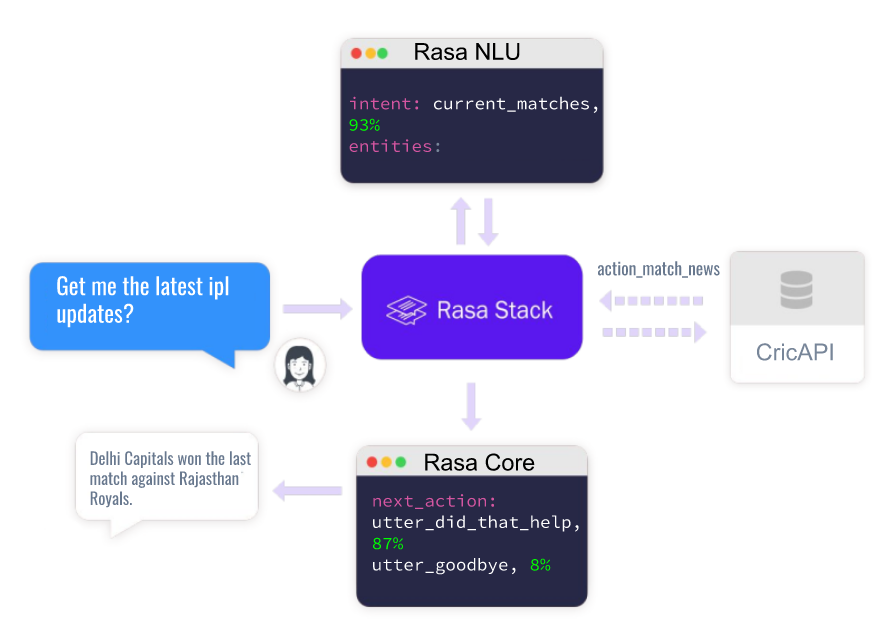
\includegraphics[width=\linewidth,keepaspectratio]{images/rasa_full4.png}
\end{center}

\end{frame}


% %%%%%%%%%%%%%%%%%%%%%%%%%%%%%%%%%%%%%%%%%%%%%%%%%%%%%%%%%%%
 % \begin{frame}[fragile]\frametitle{Architecture of chatbot}

% \begin{itemize}
% \item As soon as Rasa receives a message from the end user, it tries to predict or extract the ``intent'' and ``entities'' present in the message. This part is handled by Rasa NLU
% \item Once the user's intent is identified, the Rasa Stack performs an action called action\_match\_news to get the updates from the latest IPL match
% \item Rasa then tries to predict what it should do next. This decision is taken considering multiple factors and is handled by Rasa Core
% \item In this example, Rasa is showing the result of the most recent match to the user. It has also predicted the next action that our model should take – to check with the user whether the chatbot was able to solve his/her query
% \end{itemize}

% \end{frame}

%%%%%%%%%%%%%%%%%%%%%%%%%%%%%%%%%%%%%%%%%%%%%%%%%%%%%%%%%%%%%%%%%%%%%%%%%%%%%%%%%%
\begin{frame}[fragile]\frametitle{}
\begin{center}
{\Large Setup}


\end{center}
\end{frame}

%%%%%%%%%%%%%%%%%%%%%%%%%%%%%%%%%%%%%%%%%%%%%%%%%%%%%%%%%%%
 \begin{frame}[fragile]\frametitle{Installations}
Official Documentation: https://rasa.com/docs/core/installation/

\begin{itemize}
\item Python
\item Rasa Stack
\item Spacy Language Model
\end{itemize}

\end{frame}

% %
% %%%%%%%%%%%%%%%%%%%%%%%%%%%%%%%%%%%%%%%%%%%%%%%%%%%%%%%%%%%
 % \begin{frame}[fragile]\frametitle{Python}
% \begin{itemize}
% \item Install Anaconda 4.2.0 for Python 3.5 or Ananconda 5.2.0 for Python 3.6 
% \item Else from Python.org and then additionally numpy and scipy
% \item Ubuntu : 
% \begin{lstlisting}
% sudo apt-get install build-essential python-dev git
% \end{lstlisting}
% \item Windows Build tools: Make sure the Microsoft $VC++$ Compiler Visual Studio 2015 is installed, so python can compile any dependencies or https://visualstudio.microsoft.com/visual-cpp-build-tools/ Download the installer and select VC++ Build tools in the list.
% \end{itemize}

% Note: On main page of Anaconda is https://www.anaconda.com/distribution/ you see Python 3.7, which is problematic, gives HTTP error while creating env. I had to delete 3.7 and get 3.6. Btw, this site does not mention which Anaconda installer has which Python version. WHY? thats the most crucial info. Anyway, I have given them here.

% \end{frame}

%%%%%%%%%%%%%%%%%%%%%%%%%%%%%%%%%%%%%%%%%%%%%%%%%%%%%%%%%%%
 \begin{frame}[fragile]\frametitle{Python Environment}
\begin{itemize}
\item By installing conda, you get base or the root environment, which is the default.
\item Practical tip: DO NOT install any packages in the root. ALWAYS create and env and install inside the new env.
\item Env is needed especially for fragile packages like Python (its treated as a package) and rasa.
\item So, \lstinline|conda create -n rasa python=3.6| 
\end{itemize}

(Note: Env management is again a sour point. It creates complete copy (deeeep) of python 3.6 and all other packages inside ``envs'' folder. Goes to 1.5 GB!! Can someone optimize it?)
\end{frame}

%%%%%%%%%%%%%%%%%%%%%%%%%%%%%%%%%%%%%%%%%%%%%%%%%%%%%%%%%%%
 \begin{frame}[fragile]\frametitle{IPL bot code (for reference)}
\begin{itemize}
\item Clone repo from https://github.com/mohdsanadzakirizvi/iplbot.git
\item  ``Complete Version'' gives latest running application (Some modifications are needed, mentioned below)
\item But, WE WILL BE CODING IT FROM SCRATCH
\item Run following commands:

\begin{lstlisting}
mkdir code; cd code;mkdir data
activate rasa
pip install -r iplbot_requirements.txt
\end{lstlisting}
\item If you have environment.yml, use \lstinline|conda create -f environment.yml|
\item You may see Microsoft Visual Studio error about build tools. For that install c++ build tools exe.

\end{itemize}
\end{frame}



%%%%%%%%%%%%%%%%%%%%%%%%%%%%%%%%%%%%%%%%%%%%%%%%%%%%%%%%%%%
 \begin{frame}[fragile]\frametitle{Great for getting started: $spaCy + sklearn$}
 The spacy\_sklearn pipeline combines a few different libraries and is a popular option.

\begin{lstlisting}
python -m spacy download en_core_web_md # This will show that linking is done, but it may not have happened actually. So, do next step anyway

python -m spacy link en_core_web_md en --force
\end{lstlisting}

If any errors related to 'en', try \lstinline| python -m spacy download en| in cmd with admin permissions.
else copy \lstinline|envs\rasa\lib\site-packages\en_core_web_sm| as \lstinline|envs\rasa\lib\site-packages\spacy\data\en|

% \begin{itemize}
% \item Recommending using at least the ``medium'' sized models (\_md) instead of the spacy's default small en\_core\_web\_sm model. 
% \item Small models require less memory to run, but will somewhat reduce intent classification performance.
% \end{itemize}
% Install crf suite by 
% \begin{lstlisting}
% pip install sklearn_crfsuite
% \end{lstlisting}
\end{frame}

%%%%%%%%%%%%%%%%%%%%%%%%%%%%%%%%%%%%%%%%%%%%%%%%%%%%%%%%%%%
 \begin{frame}[fragile]\frametitle{Others}
\begin{itemize}
\item Install nb\_conda\_kernels to let Jupyter Notebook see the new env
\item Create account on cricapi.com (free, can login using Google account). Note down API Key and set it as CRICINFOAPI env variable
\end{itemize}

\end{frame}


%%%%%%%%%%%%%%%%%%%%%%%%%%%%%%%%%%%%%%%%%%%%%%%%%%%%%%%%%%%%%%%%%%%%%%%%%%%%%%%%%%
\begin{frame}[fragile]\frametitle{}
\begin{center}
{\Large Getting started \ldots}


\end{center}
\end{frame}



%%%%%%%%%%%%%%%%%%%%%%%%%%%%%%%%%%%%%%%%%%%%%%%%%%%%%%%%%%%
 \begin{frame}[fragile]\frametitle{Importing the Libraries}

\begin{lstlisting}
import rasa_nlu
import rasa_core
import spacy
\end{lstlisting}
\end{frame}


% %%%%%%%%%%%%%%%%%%%%%%%%%%%%%%%%%%%%%%%%%%%%%%%%%%%%%%%%%%%%%%%%%%%%%%%%%%%%%%%%%%
% \begin{frame}[fragile]\frametitle{}
% \begin{center}
% {\Large Rasa NLU}
% \end{center}
% \end{frame}

% %%%%%%%%%%%%%%%%%%%%%%%%%%%%%%%%%%%%%%%%%%%%%%%%%%%%%%%%%%%
 % \begin{frame}[fragile]\frametitle{Extracting User Intent from a Message}

% \begin{itemize}
% \item The first thing we want to do is figure out the intent of the user.
% \item What does he or she want to accomplish? 
% \item Let's utilize Rasa and build an NLU model to identify user intent and its related entities.
% \end{itemize}

% \end{frame}

%%%%%%%%%%%%%%%%%%%%%%%%%%%%%%%%%%%%%%%%%%%%%%%%%%%%%%%%%%%
 \begin{frame}[fragile]\frametitle{Preparing the NLU Training Data}
Training data for extracting the user intent. As you can see, the format of training data for `intent' is quite simple in Rasa. You just have to:
\begin{itemize}
\item Start the line with ``\#\# intent:intent\_name''
\item Supply all the examples in the following lines
\end{itemize}

\end{frame}

%%%%%%%%%%%%%%%%%%%%%%%%%%%%%%%%%%%%%%%%%%%%%%%%%%%%%%%%%%%
 \begin{frame}[fragile]\frametitle{NLU training file}
data/nlu\_data.md

\begin{lstlisting}
## intent:greet
- Hi
- Hey
- Hi bot
- Hey bot
- Hello
:
## intent:current_matches
- what are the current matches
- can you list the matches in ipl 2019
- which cricket match is happening right now
- which ipl match is next
- which teams are playing next in ipl
- which team will play next in ipl
:
\end{lstlisting}
\end{frame}

%%%%%%%%%%%%%%%%%%%%%%%%%%%%%%%%%%%%%%%%%%%%%%%%%%%%%%%%%%%
 \begin{frame}[fragile]\frametitle{Preparing the NLU Training Data}

\begin{itemize}
\item You can include as many examples as you want for each intent. 
\item In fact, make sure to include slangs and short forms that you use while texting. 
\item The idea is to make the chatbot understand the way we type text. 
\item Feel free to refer to the complete version where I have given plenty of examples for each intent type.
\end{itemize}

\end{frame}

%%%%%%%%%%%%%%%%%%%%%%%%%%%%%%%%%%%%%%%%%%%%%%%%%%%%%%%%%%%
 \begin{frame}[fragile]\frametitle{Defining the NLU Model Configuration}
This file lets us create a text processing pipeline in Rasa. Luckily for us, Rasa comes with two default settings based on the amount of training data we have:

\begin{itemize}
\item ``spacy\_sklearn'' pipeline if you have less than 1000 training examples
\item ``tensorflow\_embedding'' if you have a large amount of data
\end{itemize}

config/nlu\_config.yml
 
\begin{lstlisting}
language: "en"
pipeline: spacy_sklearn
\end{lstlisting}

\end{frame}

%%%%%%%%%%%%%%%%%%%%%%%%%%%%%%%%%%%%%%%%%%%%%%%%%%%%%%%%%%%
 \begin{frame}[fragile]\frametitle{Training the NLU Classifier Model}
On command line you can run following command:

\begin{lstlisting}
python -m rasa_nlu.train -c nlu_config.yml --data data/nlu_data.md -o models --fixed_model_name nlu --project current --verbose
\end{lstlisting}

\end{frame}

%%%%%%%%%%%%%%%%%%%%%%%%%%%%%%%%%%%%%%%%%%%%%%%%%%%%%%%%%%%
 \begin{frame}[fragile]\frametitle{Training the NLU Classifier Model}
 Or programmatically you can write code
 
\begin{lstlisting}
from rasa_nlu.training_data import load_data
from rasa_nlu.config import RasaNLUModelConfig
from rasa_nlu.model import Trainer
from rasa_nlu import config

# loading the nlu training samples
training_data = load_data("data/nlu_data.md")

# trainer to educate our pipeline
trainer = Trainer(config.load("config/nlu_config.yml"))

# train the model!
interpreter = trainer.train(training_data)

# store it for future use
model_directory = trainer.persist("./models/nlu", fixed_model_name="current")
\end{lstlisting}

\end{frame}

%%%%%%%%%%%%%%%%%%%%%%%%%%%%%%%%%%%%%%%%%%%%%%%%%%%%%%%%%%%
 \begin{frame}[fragile]\frametitle{Evaluating the NLU model on a random text (first way)}
 

Let's test how good our model is performing by giving it a sample text that it hasn't been trained on for extracting intent. 
\begin{lstlisting}
# A helper function for prettier output

def pprint(o):   
    print(json.dumps(o, indent=2))
    
pprint(interpreter.parse("what is happening in the cricket world these days?"))
\end{lstlisting}
 
\end{frame}

%%%%%%%%%%%%%%%%%%%%%%%%%%%%%%%%%%%%%%%%%%%%%%%%%%%%%%%%%%%
 \begin{frame}[fragile]\frametitle{Evaluating the NLU model on a random text (first way)}

\begin{lstlisting}
{
  "intent": {
    "name": "current_matches",
    "confidence": 0.5124748469776419
  },
  "entities": [],
  "intent_ranking": [
    {
      "name": "current_matches",
      "confidence": 0.5124748469776419
    },
	:
    {
      "name": "thanks",
      "confidence": 0.03056775368880194
    }
  ],
  "text": "what is happening in the cricket world these days?"
}
\end{lstlisting}
Not only does our NLU model perform well on intent extraction, but it also ranks the other intents based on their confidence scores. This is a nifty little feature that can be really useful when the classifier is confused between multiple intents.
\end{frame}

%%%%%%%%%%%%%%%%%%%%%%%%%%%%%%%%%%%%%%%%%%%%%%%%%%%%%%%%%%%
 \begin{frame}[fragile]\frametitle{Evaluating the NLU model on a random text (2nd way)}
 

Let's test how good our model is performing by giving it a sample text that it hasn't been trained on for extracting intent. You can open an iPython/Python shell and follow the following steps: 
\begin{lstlisting}
from rasa_nlu.model import Interpreter
nlu_model = Interpreter.load('./models/nlu/default/current')
nlu_model.parse('what is happening in the cricket world these days?')
\end{lstlisting}
 
\end{frame}

%%%%%%%%%%%%%%%%%%%%%%%%%%%%%%%%%%%%%%%%%%%%%%%%%%%%%%%%%%%
 \begin{frame}[fragile]\frametitle{Evaluating the NLU model on a random text (2nd way)}

\begin{lstlisting}
{'intent': {'name': 'current_matches', 'confidence': 0.5124748469776419},
 'entities': [],
 'intent_ranking': [{'name': 'current_matches',
   'confidence': 0.5124748469776419},
  {'name': 'greet', 'confidence': 0.26316772065557126},
  {'name': 'goodbye', 'confidence': 0.09389099823148171},
  {'name': 'affirm', 'confidence': 0.06686974145943789},
  {'name': 'deny', 'confidence': 0.03302893898706549},
  {'name': 'thanks', 'confidence': 0.03056775368880194}],
 'text': 'what is happening in the cricket world these days?'}
\end{lstlisting}

\end{frame}



%%%%%%%%%%%%%%%%%%%%%%%%%%%%%%%%%%%%%%%%%%%%%%%%%%%%%%%%%%%
 \begin{frame}[fragile]\frametitle{Evaluating the NLU model on a test data}
 
    \begin{columns}
    \begin{column}[t]{0.5\linewidth}
Let us now evaluate it on a test data set. However, for our purpose let's evaluate it on the data at hand i.e nlu\_data.md
\begin{lstlisting}
from rasa_nlu.evaluate import run_evaluation
run_evaluation("data/nlu_data.md", model_directory)
\end{lstlisting}

We get an Intent Confusion matrix with the with various evaluation results.
    \end{column}
    \begin{column}[t]{0.5\linewidth}
\begin{lstlisting}
{'intent_evaluation': {'predictions': [{'text': 'Bye',
    'intent': 'goodbye',
    'predicted': 'goodbye',
    'confidence': 0.9627578046567274},
   {'text': 'Goodbye',
    'intent': 'goodbye',
    'predicted': 'goodbye',
    'confidence': 0.8796549909963912},
	:
   'precision': 1.0,
   'f1_score': 1.0,
   'accuracy': 1.0}}}
\end{lstlisting}
    \end{column}
  \end{columns}
\end{frame}

%%%%%%%%%%%%%%%%%%%%%%%%%%%%%%%%%%%%%%%%%%%%%%%%%%%%%%%%%%%
 \begin{frame}[fragile]\frametitle{}
 \begin{center}
{\Large Rasa Core}
\end{center}
\end{frame}

%%%%%%%%%%%%%%%%%%%%%%%%%%%%%%%%%%%%%%%%%%%%%%%%%%%%%%%%%%%
 \begin{frame}[fragile]\frametitle{Making Interactive Conversations}

 
\begin{itemize}
\item  One of the most important aspects of a chatbot application is its ability to be interactive.
 
\item Think of the simplest conversation our chatbot can have with a user. What would be the flow of such a conversation?
\end{itemize}
\begin{lstlisting}
Me: Hi

Iplbot: Hey! How may I help you?

Me: What was the result of the last match?

Iplbot: Here are some IPL quick info: 1.The match between Rajasthan Royals and Delhi Capitals was recently held and Delhi Capitals won. 2.The next match is Warriors vs Titans on 22 April 2019

Iplbot: Did that help you?

Me: yes, thank you!

Iplbot: Glad that I could help!
\end{lstlisting}
\end{frame}

%%%%%%%%%%%%%%%%%%%%%%%%%%%%%%%%%%%%%%%%%%%%%%%%%%%%%%%%%%%
 \begin{frame}[fragile]\frametitle{Making Interactive Conversations}

Let's see how we can teach a simple conversation like that to Rasa:

\begin{lstlisting}
## news path 1
* greet
  - utter_greet
* current_matches
  - action_match_news
  - utter_did_that_help
* affirm or thanks
  - utter_gratitude
* goodbye
  - utter_goodbye
\end{lstlisting}

The general format is:

\begin{lstlisting}
## news path 1           <--- story name for debugging purposes
* greet                  <--- intent detected from the user
  - utter_greet          <--- what action the bot should take
* current_matches        <--- the following intent in the conversation
\end{lstlisting}

This is called a user story path. I have provided a few stories in the data/stories.md file for your reference. This is the training data for Rasa Core.
\end{frame}


%%%%%%%%%%%%%%%%%%%%%%%%%%%%%%%%%%%%%%%%%%%%%%%%%%%%%%%%%%%
 \begin{frame}[fragile]\frametitle{Making Interactive Conversations}


\begin{itemize}
\item We will teach chatbot to make responses by training a dialogue management model using Rasa Core.
\item For dialog training, Rasa has 4 main components
\begin{itemize}
\item Domain(config/domain.yml)
\item Stories (data/stories.md)
\item Policies (config/policy.yml)
\item Custom Actions (actions.py)
\end{itemize}

\end{itemize}
\end{frame}

%%%%%%%%%%%%%%%%%%%%%%%%%%%%%%%%%%%%%%%%%%%%%%%%%%%%%%%%%%%
 \begin{frame}[fragile]\frametitle{Writing Stories}
The way it works is:

\begin{itemize}
\item Give some examples of sample story paths that the user is expected to follow
\item Rasa Core combines them randomly to create more complex user paths
\item It then builds a probabilistic model out of that. This model is used to predict the next action Rasa should take
\end{itemize}


\end{frame}

%%%%%%%%%%%%%%%%%%%%%%%%%%%%%%%%%%%%%%%%%%%%%%%%%%%%%%%%%%%
 \begin{frame}[fragile]\frametitle{Writing Stories}


\begin{center}
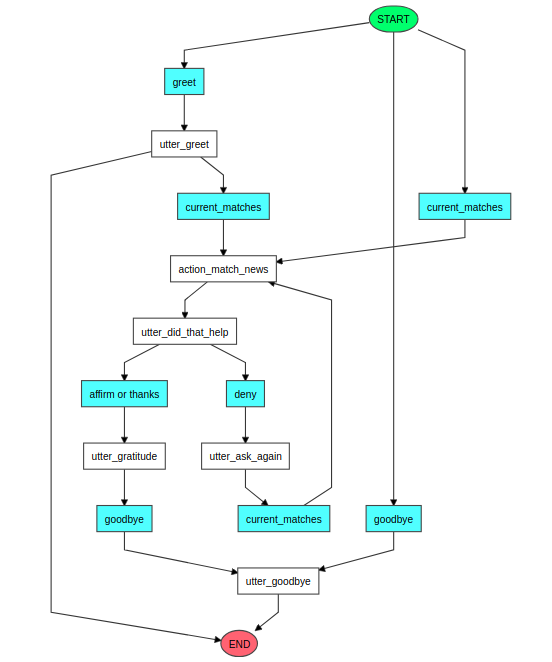
\includegraphics[width=0.55\linewidth,keepaspectratio]{images/conversation_flow.png}
\end{center}
\end{frame}

%%%%%%%%%%%%%%%%%%%%%%%%%%%%%%%%%%%%%%%%%%%%%%%%%%%%%%%%%%%
 \begin{frame}[fragile]\frametitle{Writing Stories}

 The illustration might look complicated, but it's simply listing out various possible user stories that I have taught Rasa. Here are a few things to note from the above graph:
 
 
\begin{itemize}
\item Except for the START and END boxes, all the colored boxes indicate user intent
\item All the white boxes are actions that the chatbot performs
\item  Arrows indicate the flow of the conversation
\item  action\_match\_news is where we hit the CricAPI to get IPL information
\end{itemize}
\end{frame}


%%%%%%%%%%%%%%%%%%%%%%%%%%%%%%%%%%%%%%%%%%%%%%%%%%%%%%%%%%%
\begin{frame}[fragile]\frametitle{Writing Stories}

data/stories.md

\begin{lstlisting}
## news path 1
* greet
  - utter_greet
* current_matches
  - action_match_news
  - utter_did_that_help
* affirm or thanks
  - utter_gratitude
* goodbye
  - utter_goodbye
:
\end{lstlisting}

Now, generate a similar graph for your stories using the following command:

\begin{lstlisting}
python -m rasa_core.visualize -d domain.yml -s data/stories.md -o graph.html
\end{lstlisting}

This is very helpful when debugging the conversational flow of the chatbot.

\end{frame}

%%%%%%%%%%%%%%%%%%%%%%%%%%%%%%%%%%%%%%%%%%%%%%%%%%%%%%%%%%%
 \begin{frame}[fragile]\frametitle{Defining the Domain}

The domain is the world of your chatbot. It contains everything the chatbot should know, including:
 
 
\begin{itemize}
\item All the actions it is capable of doing
\item The intents it should understand
\item The template of all the utterances it should tell the user, and much more
\end{itemize}
\end{frame}

%%%%%%%%%%%%%%%%%%%%%%%%%%%%%%%%%%%%%%%%%%%%%%%%%%%%%%%%%%%
 \begin{frame}[fragile]\frametitle{Defining the Domain}

config/domain.yml
\begin{lstlisting}
actions:
- utter_greet
- utter_did_that_help
- utter_goodbye
- action_match_news
- utter_default
- utter_gratitude
- utter_ask_again

intents:
- goodbye
- greet
- thanks
- current_matches
- affirm
- deny

:
\end{lstlisting}


\end{frame}


%%%%%%%%%%%%%%%%%%%%%%%%%%%%%%%%%%%%%%%%%%%%%%%%%%%%%%%%%%%
 \begin{frame}[fragile]\frametitle{Defining the Domain}

config/domain.yml
\begin{lstlisting}
:

templates:
  utter_greet:
  - text: "Hey! What can I do for you?"
  utter_did_that_help:
  - text: "Did that help you?"
  - text: "I hope that solved your query"
  utter_goodbye:
  - text: "Bye"
  utter_default:
  - text: "I am sorry, I didn't get that. Could you please repeat your query?"
  - text: "I am not sure what you are aiming for."
  utter_gratitude:
  - text: "Glad that I could be of help to you!\nBye"
  utter_ask_again:
  - text: "Okay! Let's start again, please tell me what do you need?"
  - text: "No issues! Let's try this again.\n Please repeat your query?"
\end{lstlisting}


\end{frame}

%%%%%%%%%%%%%%%%%%%%%%%%%%%%%%%%%%%%%%%%%%%%%%%%%%%%%%%%%%%
 \begin{frame}[fragile]\frametitle{Setting Policies}

 
\begin{itemize}
\item Rasa Core generates the training data for the conversational part using the stories we provide. 
\item It also lets you define a set of policies to use when deciding the next action of the chatbot. \item These policies are defined in the policies.yml file.
\item Else these params can be passed, while training, to respective Policy constructors
\end{itemize}

config/policies.yml

\begin{lstlisting}
policies:
  - name: KerasPolicy
    epochs: 100
    max_history: 5
  - name: FallbackPolicy
    fallback_action_name: 'action_default_fallback'
  - name: MemoizationPolicy
    max_history: 5
\end{lstlisting}
\end{frame}

%%%%%%%%%%%%%%%%%%%%%%%%%%%%%%%%%%%%%%%%%%%%%%%%%%%%%%%%%%%
 \begin{frame}[fragile]\frametitle{Setting Policies}

 
\begin{itemize}
\item KerasPolicy uses a neural network implemented in Keras to select the next action. The default architecture is based on an LSTM (Long Short Term Memory) model
\item MemoizationPolicy memorizes the conversations in your training data. It predicts the next action with confidence 1.0 if this exact conversation exists in the training data, otherwise, it predicts `None' with confidence 0.0
\item FallbackPolicy invokes a fallback action if the intent recognition has confidence below nlu\_threshold or if none of the dialogue policies predict action with confidence higher than core\_threshold
\item One important hyperparameter for Rasa Core policies is the max\_history. This controls how much dialogue history the model looks at to decide which action to take next
\end{itemize}

\end{frame}

%%%%%%%%%%%%%%%%%%%%%%%%%%%%%%%%%%%%%%%%%%%%%%%%%%%%%%%%%%%
 \begin{frame}[fragile]\frametitle{Custom Actions}

 
\begin{itemize}
\item Using CricAPI for fetching IPL related news. It is free for 100 requests per day, which (I hope) is more than enough to satiate that cricket crazy passion you have.
\item You need to first signup on the website to get access to their API: https://www.cricapi.com/
\item You should be able to see your API Key once you are logged in:
\end{itemize}

\end{frame}

%%%%%%%%%%%%%%%%%%%%%%%%%%%%%%%%%%%%%%%%%%%%%%%%%%%%%%%%%%%
 \begin{frame}[fragile]\frametitle{Custom Actions}

\begin{center}
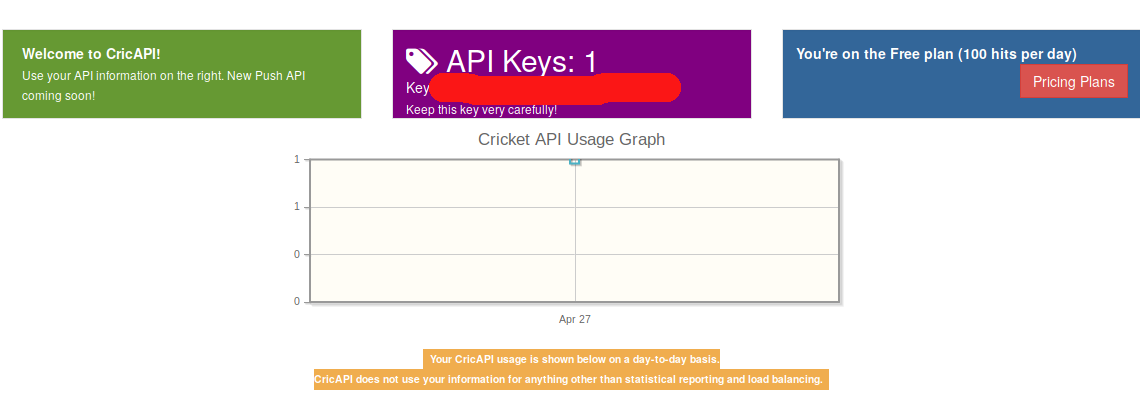
\includegraphics[width=\linewidth,keepaspectratio]{images/lala-1140x399.png}
\end{center}

Modifications to original code:

\begin{itemize}
\item Instead of showing API key here it has been stored in ENV variable and fetched here
\item  Key "toss\_winner\_team" was subsituted into depreceated key
\end{itemize}

\end{frame}


%%%%%%%%%%%%%%%%%%%%%%%%%%%%%%%%%%%%%%%%%%%%%%%%%%%%%%%%%%%
 \begin{frame}[fragile]\frametitle{Custom Actions}

 actions.py

\begin{lstlisting}
# -*- coding: utf-8 -*-
from __future__ import absolute_import
from __future__ import division
from __future__ import print_function
from __future__ import unicode_literals
from datetime import datetime

import logging
import requests
import json
import os
from rasa_core_sdk import Action

logger = logging.getLogger(__name__)

API_URL = "https://cricapi.com/api/"
API_KEY = os.environ.get('CRICINFOAPI')
\end{lstlisting}
\end{frame}

%%%%%%%%%%%%%%%%%%%%%%%%%%%%%%%%%%%%%%%%%%%%%%%%%%%%%%%%%%%
 \begin{frame}[fragile]\frametitle{Custom Actions}

actions.py

\begin{lstlisting}
class ApiAction(Action):
    def name(self):
        return "action_match_news"

    def run(self, dispatcher, tracker, domain):
        print(API_URL + "matches" + "?apikey=" + API_KEY)
        res = requests.get(API_URL + "matches" + "?apikey=" + API_KEY) #, verify=False
        if res.status_code == 200:
            data = res.json()["matches"]
            recent_match = data[0]
            upcoming_match = data[1]
            upcoming_match["date"] = datetime.strptime(upcoming_match["date"], "%Y-%m-%dT%H:%M:%S.%fZ")
            next_date = upcoming_match["date"].strftime("%d %B %Y")

\end{lstlisting}
\end{frame}

%%%%%%%%%%%%%%%%%%%%%%%%%%%%%%%%%%%%%%%%%%%%%%%%%%%%%%%%%%%
 \begin{frame}[fragile]\frametitle{Custom Actions}

actions.py

\begin{lstlisting}
class ApiAction(Action):

    def run(self, dispatcher, tracker, domain):
			:

            out_message = "Here some IPL quick info: 1.The match between {} and {} was recently held and {} won the toss.".format(recent_match["team-1"], recent_match["team-2"], recent_match["toss_winner_team"])

            dispatcher.utter_message(out_message)

            out_message = "2.The next match is {} vs {} on {}".format(upcoming_match["team-1"], upcoming_match["team-2"], next_date)

            dispatcher.utter_message(out_message)

            return []
\end{lstlisting}
\end{frame}

%%%%%%%%%%%%%%%%%%%%%%%%%%%%%%%%%%%%%%%%%%%%%%%%%%%%%%%%%%%
 \begin{frame}[fragile]\frametitle{Custom Actions}

\begin{itemize}
\item Need endpoints yml to execute the actions server.
\item Note: If you have external API call, like REST, need to have ``webhook'' word at the end, else nothing.
\item My own query on this topic: https://forum.rasa.com/t/rasa-core-sdk-not-working/9228
\end{itemize}

endpoints.yml
\begin{lstlisting}
action_endpoint:
  url: http://localhost:5055/webhook

core_endpoint:
  url: http://localhost:5005
\end{lstlisting}
\end{frame}

%%%%%%%%%%%%%%%%%%%%%%%%%%%%%%%%%%%%%%%%%%%%%%%%%%%%%%%%%%%
 \begin{frame}[fragile]\frametitle{Custom Actions}

 In a separate shell (cmd for Windows):
 
\begin{itemize}
\item \lstinline|activate rasa|
\item Come to directory where actions.py is and then run
\item \lstinline|python -m rasa_core_sdk.endpoint --actions actions|
\end{itemize}

This way, custom action server starts \ldots
\end{frame}

%%%%%%%%%%%%%%%%%%%%%%%%%%%%%%%%%%%%%%%%%%%%%%%%%%%%%%%%%%%
 \begin{frame}[fragile]\frametitle{Visualizing the Training Data}


\begin{lstlisting}
from IPython.display import Image, display
from rasa_core.agent import Agent
%matplotlib inline

agent = Agent('config/domain.yml')
agent.visualize("data/stories.md", "story_graph.png", max_history=2)
i = Image(filename="story_graph.png")
display(i)
\end{lstlisting}

\end{frame}

%%%%%%%%%%%%%%%%%%%%%%%%%%%%%%%%%%%%%%%%%%%%%%%%%%%%%%%%%%%
 \begin{frame}[fragile]\frametitle{Training a Dialogue Model}


\begin{itemize}
\item You can train the model using the following command:

\item \lstinline|python -m rasa_core.train -d domain.yml -s data/stories.md -o models/current/dialogue -c policies.yml|
\end{itemize}

\end{frame}

%%%%%%%%%%%%%%%%%%%%%%%%%%%%%%%%%%%%%%%%%%%%%%%%%%%%%%%%%%%
 \begin{frame}[fragile]\frametitle{Training a Dialog Model}

Or do it programmatically as:

\begin{lstlisting}
from rasa_core.policies import FallbackPolicy, KerasPolicy, MemoizationPolicy
from rasa_core.agent import Agent

# this will catch predictions the model isn't very certain about
# there is a threshold for the NLU predictions as well as the action predictions
fallback = FallbackPolicy(fallback_action_name="utter_unclear",
                          core_threshold=0.2,
                          nlu_threshold=0.1)

\end{lstlisting}

\end{frame}

%%%%%%%%%%%%%%%%%%%%%%%%%%%%%%%%%%%%%%%%%%%%%%%%%%%%%%%%%%%
 \begin{frame}[fragile]\frametitle{Training a Dialog Model}

\begin{lstlisting}

agent = Agent('domain.yml', policies = [MemoizationPolicy(max_history=2), KerasPolicy(epochs = 200,validation_split = 0.2)])
# loading our neatly defined training dialogues
training_data = agent.load_data('data/stories.md')

agent.train(training_data)
# FOLOWING WAY has been deprecated, move these params to KerasPolicy
# agent.train(
#     training_data,
#     validation_split=0.2,
#     epochs=200
# )

agent.persist('models/current/dialogue')
\end{lstlisting}

\end{frame}

%%%%%%%%%%%%%%%%%%%%%%%%%%%%%%%%%%%%%%%%%%%%%%%%%%%%%%%%%%%%%%%%%%%%%%%%%%%%%%%%%%
\begin{frame}[fragile]\frametitle{}
\begin{center}
{\Large Running: Talk to your Bot}

\end{center}
\end{frame}



%%%%%%%%%%%%%%%%%%%%%%%%%%%%%%%%%%%%%%%%%%%%%%%%%%%%%%%%%%%
 \begin{frame}[fragile]\frametitle{Talk to your Bot}

So we have the chatbot ready. It's time to chat.

One way is to run following command in shell (windows cmd) 
\begin{itemize}
\item activate the environment,
\item Come to directory where actions.py is and then run
\item \lstinline|python -m rasa_core.run -d models/current/dialogue -u models/current/nlu --endpoints endpoints.yml|
\end{itemize}

\end{frame}

%%%%%%%%%%%%%%%%%%%%%%%%%%%%%%%%%%%%%%%%%%%%%%%%%%%%%%%%%%%
 \begin{frame}[fragile]\frametitle{Talk to your Bot}

Or do it programmatically as:

Both approaches expect rasa core sdk server running in a separate window, else 
\lstinline|python -m rasa_core_sdk.endpoint --actions actions|


\begin{lstlisting}
import IPython
from IPython.display import clear_output
from rasa_core.agent import Agent
from rasa_core.interpreter import NaturalLanguageInterpreter
from rasa_core.utils import EndpointConfig

def load_assistant():
    messages = ["Hi! Chat here. Type 'stop' to end"]
    interpreter = NaturalLanguageInterpreter.create(model_directory)
    endpoint = EndpointConfig('http://localhost:5055/webhook')
    agent = Agent.load('models/current/dialogue', interpreter=interpreter, action_endpoint = endpoint)
    print("Your bot is ready to talk! Type your messages here or send 'stop'")
    while True:
        a = input()
        if a == 'stop':
            break
        responses = agent.handle_text(a)
        for response in responses:
            print(response["text"])
\end{lstlisting}

\end{frame}

%%%%%%%%%%%%%%%%%%%%%%%%%%%%%%%%%%%%%%%%%%%%%%%%%%%%%%%%%%%
 \begin{frame}[fragile]\frametitle{Talk to your Bot}

\begin{lstlisting}
load_assistant() 

Your bot is ready to talk! Type your messages here or send 'stop'
hi
Hey! What can I do for you?
What are recent matches?
Here some IPL quick info: 1.The match between Mumbai Indians and Sunrisers Hyderabad was recently held and Mumbai Indians won the toss.
2.The next match is Kings XI Punjab vs Kolkata Knight Riders on 03 May 2019
Did that help you?
stop
\end{lstlisting}

\end{frame}

%%%%%%%%%%%%%%%%%%%%%%%%%%%%%%%%%%%%%%%%%%%%%%%%%%%%%%%%%%%
 \begin{frame}[fragile]\frametitle{Conclusion and next}

\begin{itemize}
\item We utilized the capabilities of Rasa NLU and Rasa Core to create a bot with minimum training data.
\item Try to use different pipelines in Rasa Core, explore more Policies, fine-tune those models,
\item Check out what other features CricAPI provides, etc.
\item Other APIs
\item Slot filling
\item Different languages (Hindi bot?) 
\end{itemize}

\end{frame}